\subsubsection{Terminologie}

\vspace{0.5cm}

\begin{theo}[Orthogonale en orthonormale basissen]{theo:orthogonale_orthonormale_basissen}
    We spreken van een orthogonale, respectievelijk orthonormale basis als de basisvectoren $\{a_1, \ldots, a_n\}$ orthogonaal, respectievelijk orthonormaal zijn. Als een basis niet orthogonaal is, spreken we van een scheve basis.
\end{theo}

\begin{theo}[Grammatrix]{theo:grammatrix}
    Voor een basis $\{a_1, \ldots, a_n\}$ van deelruimte $\mathcal{D}$ en twee vectoren $v, w \in \mathcal{D}$ ontbonden als
    \begin{equation*}
            v = \sum_{i=1}^{n} \alpha_i a_i, \
            w = \sum_{i=1}^{n} \beta_i a_i
    \end{equation*}
    geldt dat het inwendig product ($( v, w ) = v^*w$) van $v$ en $w$ gelijk is aan
    \begin{align*}
        ( v, w ) 
            = \left( \sum_{i=1}^{n} \alpha_i a_i^* \right)\left( \sum_{i=1}^{n} \beta_i a_i \right) 
            = 
                \begin{bmatrix} \alpha_1 & \cdots & \alpha_n \end{bmatrix} 
                \underbrace{\begin{bmatrix} ( a_1, a_1 ) & \cdots & ( a_1, a_n ) \\ \vdots & \ddots & \vdots \\ ( a_n, a_1 ) & \cdots & ( a_n, a_n ) \end{bmatrix}}_{G} 
                \begin{bmatrix} \beta_1 \\ \vdots \\ \beta_n \end{bmatrix}
            = \alpha^* G \beta
    \end{align*}
    waarbij deze G de zogenaamde \emph{grammatrix} is horende bij de basis $\{a_1, \ldots, a_n\}$.
\end{theo}

\begin{pro}[Grammatrix]{pro:grammatrix}
    \begin{itemize}
        \item Is de basis orthogonaal, dan is de grammatrix diagonaal.
        \item Is de basis orthonormaal, dan is de grammatrix de eenheidsmatrix.
    \end{itemize}
\end{pro}

\begin{theo}[Projector]{theo:projector}
    Een \emph{projector} is een matrix $P \in \mathbb{C}^{m \times m}$ die idempotent is, dit is $P^2 = P$. Matrix $P$ projecteert een vector op de ruimte $\mathcal{R}(P)$, waarbij de richting bepaald wordt door de nullspace $\mathcal{N}(P)$. Stel $v \in \mathbb{C}^m$ een willekeurige vector en $P \in \mathbb{C}^{m \times m}$ een projector, dan is $Pv \in \mathcal{R}(P)$ volgens de definitie van het bereik, en is $(I - P)v \in \mathcal{N}(P)$, omdat:
    \begin{equation*}
        P(I - P)v = (P - P^2)v \overset{P^2 = P}{=} (P-P)v = 0.
    \end{equation*}
    We kunnen dus $v$ (uniek) ontbinden in componenten volgens $\mathcal{R}(P)$ en $\mathcal{N}(P)$ als
    % \begin{equation*}
        $v = Pv + (I - P)v$.
    % \end{equation*}
\end{theo}

\newpage

% \begin{app}[Projector]{app:projector}
%     Stel $v \in \mathbb{C}^m$ een willekeurige vector en $P \in \mathbb{C}^{m \times m}$ een projector, dan is $Pv \in \mathcal{R}(P)$ volgens de definitie van het bereik, en is $(I - P)v \in \mathcal{N}(P)$, omdat 
%     \begin{equation*}
%         P(I - P)v = (P - P^2)v \overset{P^2 = P}{=} (P-P)v = 0
%     \end{equation*}
%     We kunnen dus $v$ ontbinden in componenten volgens $\mathcal{R}(P)$ en $\mathcal{N}(P)$ als
%     \begin{equation*}
%         v = Pv + (I - P)v
%     \end{equation*}
%     Deze ontbinding is uniek.
% \end{app}

\begin{pro}[Projector]{pro:projector}
    \begin{itemize}
        \item Als $v \in \mathcal{R}(P)$, dan is $Pv = v$.
        \item $\mathcal{R}(P) \cap \mathcal{N}(P) = \{0\}$.
        \item $\text{dim}(\mathcal{R}(P)) + \text{dim}(\mathcal{N}(P)) = m$.
        \item De ontbinding in componenten volgens $\mathcal{R}(P)$ en $\mathcal{N}(P)$ is uniek.
    \end{itemize}
\end{pro}

\begin{prf}[Projector]{prf:projector}
    \begin{itemize}
        \item Als $v \in \mathcal{R}(P)$, dan $\exists u: v = Pu$, en dus is $Pv = P^2u = Pu = v$.
        \item Stel $x \in \mathcal{R}(P)$ en $x \in \mathcal{N}(P)$. Er volgt dat $x = Px = 0$.
        \item Dit volgt uit de eerste dimensiestelling en vorige eigenschap.
        \item Stel $v = x_1 + y_1 = x_2 + y_2$, met $x_1, x_2 \in \mathcal{R}(P)$ en $y_1, y_2 \in \mathcal{N}(P)$. Er geldt voor $i \in {1,2}$ dat $Pv = Px_i + Py_i = x_i$. Hieruit volgt dat $x_1 = x_2$.
    \end{itemize}
\end{prf}

\begin{theo}[Complementaire projector]{theo:complementaire_projector}
    Stel $P$ een projector, dan is $\tilde{P} = I - P$ de \emph{complementaire projector} van $P$. Hierbij geldt:
    \begin{equation*}
        \mathcal{R}(P) = \mathcal{N}(I-P) = \mathcal{N}(\tilde{P})  \quad \text{en} \quad \mathcal{N}(P) = \mathcal{R}(I-P) = \mathcal{R}(\tilde{P}).
    \end{equation*}
    De ontbinding kan geschreven worden als 
    \begin{equation*}
        v = \underbrace{(I - \tilde{P})v}_{\in \mathcal{R}(P)} + \underbrace{\tilde{P}v}_{\in \mathcal{N}(P)}.
    \end{equation*}
    Matrix $\tilde{P}$ projecteert dus op $\mathcal{N}(P)$ waarbij de richting bepaald wordt door $\mathcal{R}(P)$, zie verder onderstaande figuur.
    \begin{center}
        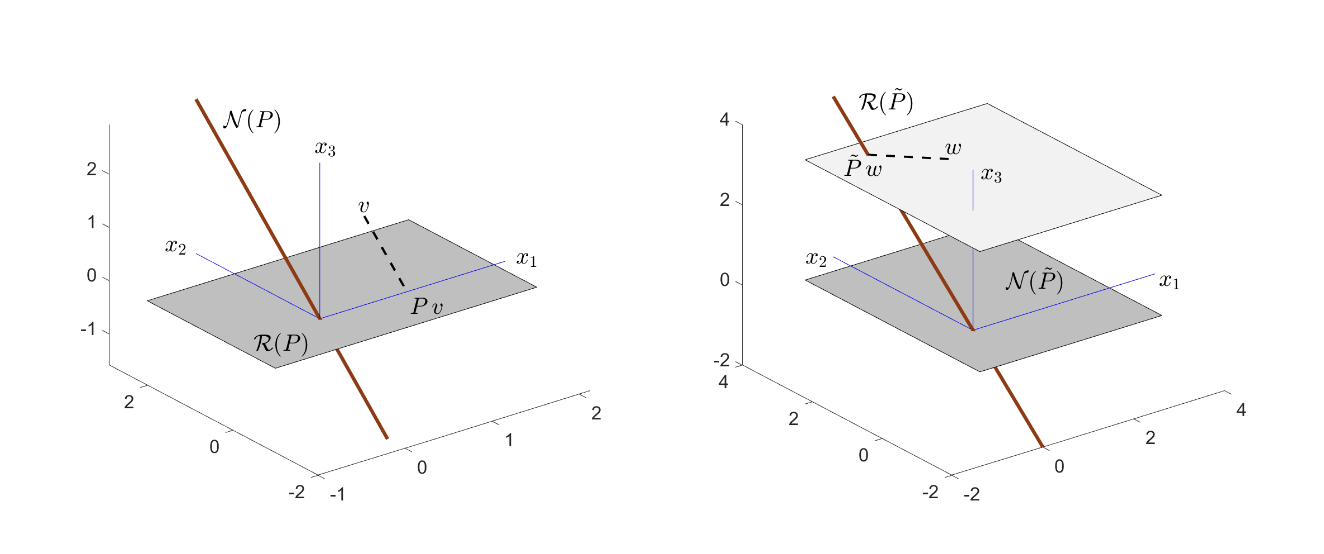
\includegraphics[width=0.75\textwidth]{Images/projectorencomplementaireprojector.png}
    \end{center}
\end{theo}

\newpage

\begin{theo}[Orthogonale projector]{theo:orthogonale_projector}
    Een projector $P$ is orthogonaal indien $\mathcal{R}(P)$ en $\mathcal{N}(P)$ onderling orthogonale ruimte zijn, m\@.a\@.w\@.
    \begin{equation*}
        P \ \text{is een orthogonale projector} \ \Leftrightarrow \ P = P^*
    \end{equation*} 
    Een projector die niet orthogonaal is, noemen we een scheve projector.
\end{theo}

% \begin{pro}[Orthogonale projector]{pro:orthogonale_projector}
%     Een projector $P$ is orthogonaal als en alleen als $P = P^*$.
% \end{pro}

\begin{prf}[Orthogonale projector]{prf:orthogonale_projector}
    ``$\Rightarrow$'': Beschouw een orthonormale basis $\{q_1, \ldots, q_n\}$ van $\mathcal{R}(P)$ en een orthonormale basis $\{q_{n+1}, \ldots, q_m\}$ van $\mathcal{N}(P)$. Omdat volgens de definitie beide ruimten orthogonaal zijn, volgt dat
    \begin{equation*}
        Q = \begin{bmatrix} q_1 & \cdots & q_n & q_{n+1} & \cdots & q_m \end{bmatrix}
    \end{equation*}
     een unitaire matrix is, m\@.a\@.w\@. $Q^*Q = QQ^* = \mathbb{I}_m$. We verkrijgen:
    \begin{equation*}
        PQ = \begin{bmatrix} q_1 & \cdots & q_n &0 & \cdots & 0 \end{bmatrix} \ \Rightarrow \ Q^*PQ = \begin{bmatrix} I_n & 0 \\ 0 & 0 \end{bmatrix}.
    \end{equation*}
    Vermits $Q^*PQ$ dus reëel is, geldt:
    \begin{equation*}
        Q^*PQ = (Q^*PQ)^* = Q^*P^*Q
    \end{equation*}
    waaruit het gestelde volgt. \\

    ``$\Leftarrow$'': Neem willekeurige $x = Pu \in \mathcal{R}(P)$ en $y \in \mathcal{N}(P)$. Dan is:
    \begin{equation*}
        ( x, y ) = x^*y = (Pu)^*y = u^*P^*y= u^*Py = 0.
    \end{equation*}
    De ruimten $\mathcal{R}(P)$ en $\mathcal{N}(P)$ zijn dus orthogonaal.
    \vspace{-0.3cm}
\end{prf}

\subsubsection{QR-factorisatie}

\vspace{0.5cm}

\begin{alg}[Gram-Schmidt orthogonalisatie]{alg:Gram-Schmidt}
    \vspace{-0.3cm}
    % \begin{minipage}{0.58\textwidth}
    %     Vertrekkende van de kolommen van $A$ bepalen we de kolommen van $\hat{Q}$ en de kolommen van $\hat{R}$ in opeenvolgende stappen. In stap $j$ bepalen we de $j$-de kolom van $\hat{R}$.
    %     \begin{itemize}
    %         \item stap 1: $r_{11} = \|a_1\|_2$ en $q_1 = a_1 / r_{11}$.
    %         \item stap $j$: Stel $q_1,q_2,\ldots,q_{j-1}$ en de $j-1$ eerste kolommen van $\hat{R}$ gekend. Dan is:
    %         \begin{equation*}
    %             a_j = \sum_{i=1}^{j} r_{ij} q_i.
    %         \end{equation*}
    %         Wegens de orthogonaliteit van vectoren $q_i$ geldt: $q_i^* a_j = r_{ij}$. Verder is:
    %         \begin{equation*}
    %             r_{ji}q_j = a_j - \sum_{i=1}^{j-1} r_{ij} q_i := v_j,
    %         \end{equation*}
    %         dus $q_j$ is gekend op een constante na en we weten dat $\|q_j\|_2 = 1$. We kiezen nu $r_{jj} = \|v_j\|_2$ en $q_j = v_j / r_{jj}$.
    %     \end{itemize}
    % \end{minipage}
    % \begin{minipage}{0.4\textwidth}
    \begin{tcolorbox}[colback=white, colframe=gray, arc=0mm] 
        \begin{algorithmic}[1]
        \For{$j = 1$ to $n$}
            \State $v_j = a_j$
            \For{$i = 1$ to $j - 1$}
                \State $r_{ij} = q_i^* a_j$
                \State $v_j = v_j - r_{ij} q_i$ \ $(= a_j - P_{<q_1,\ldots,q_{j-1}>} a_j)$
            \EndFor
            \State $r_{jj} = \|v_j\|_2$
            \State $q_j = v_j / r_{jj}$
        \EndFor
        \end{algorithmic}
    \end{tcolorbox}
    % \end{minipage}
    \vspace{-0.3cm}
\end{alg}

\begin{alg}[Gewijzigde Gram-Schmidt orthogonalisatie]{alg:gewijzigde_Gram-Schmidt}
    \vspace{-0.3cm}
    \begin{tcolorbox}[colback=white, colframe=gray, arc=0mm] 
        \begin{algorithmic}[1]
        \For{$j = 1$ to $n$}
            \State $v_j = a_j$
            \For{$i = 1$ to $j - 1$}
                \State $r_{ij} = q_i^* \boldsymbol{v_j}$ \ ($a_j \ \rightarrow \ v_j$)
                \State $v_j = v_j - r_{ij} q_i$ \ $(= (\mathbb{I} - P_{<q_{j - 1}>})\ldots(\mathbb{I} - P_{<q_{2}>})(\mathbb{I} - P_{<q_{1}>})a_j)$
            \EndFor
            \State $r_{jj} = \|v_j\|_2$
            \State $q_j = v_j / r_{jj}$
        \EndFor
        \end{algorithmic}
    \end{tcolorbox}
    \vspace{-0.3cm}
\end{alg}

\begin{app}[Herorthogonalisatie van Gram-Schmidt]{app:herorthogonalisatie}
    De Gram-Schmidt orthogonalisatie is numeriek instabiel. Dit kan verholpen worden door herorthogonalisatie, hieronder twee varianten waarvan de eerste de meest gebruikte is.
    \begin{enumerate}
            % \begin{tcolorbox}[colback=white, colframe=gray, arc=0mm] 
            %     \begin{algorithmic}[1]
                % \State $v_j = a_j$
                % \For{$j = 1$ to $j-1$}
                %     \State $r_{ij} = q_i^* v_j$
                %     \State $v_j = v_j - r_{ij} q_i$
                % \EndFor
                % \State
                % \State $w_j = v_j$
                % \For{$i = 1$ to $j -1$}
                %     \State $s_{ij} = q_i^* w_j$
                %     \State $v_j = v_j - s_{ij} q_i$
                %     \State $r_{ij} = r_{ij} + s_{ij}$
                % \EndFor
            %     \end{algorithmic}
            % \end{tcolorbox}
        \item \textbf{Stapsgewijze variant}: Het klassieke Gram-Schmidt algoritme (Algoritme~\ref{alg:Gram-Schmidt}) wordt lichtelijk aangepast:
                    \begin{tcolorbox}[colback=white, colframe=gray, arc=0mm] 
                    \begin{algorithmic}[1]
                    \For{$j = 1$ to $n$}
                        \State \textcolor{red}{$v_j = a_j$}
                        \For{$j = 1$ to $j-1$}
                            \State \textcolor{red}{$r_{ij} = q_i^* v_j$}
                            \State \textcolor{red}{$v_j = v_j - r_{ij} q_i$}
                        \EndFor
                        \State
                        \State \textcolor{red}{$w_j = v_j$}
                        \For{$i = 1$ to $j -1$}
                            \State \textcolor{red}{$s_{ij} = q_i^* w_j$}
                            \State \textcolor{red}{$v_j = v_j - s_{ij} q_i$}
                            \State \textcolor{red}{$r_{ij} = r_{ij} + s_{ij}$}
                        \EndFor
                        \State
                        \State $r_{jj} = \|v_j\|_2$
                        \State $q_j = v_j / r_{jj}$
                    \EndFor
                    \end{algorithmic}
                \end{tcolorbox}
        \item \textbf{Simultane variant}: Na het berekenen van de onvolledige QR-factorisatie, die resulteert in factoren $\hat{Q}_1$ en $\hat{R}_1$ wordt het algoritme opnieuw toegepast met als input de eerste factor, wat resulteert in $\hat{Q}_1 \approx \hat{Q}_2\hat{R}_2$. We bepalen dan $\hat{Q} = \hat{Q}_2$ en $\hat{R} = \hat{R}_2\hat{R}_1$. Bij het gewijzigde algoritme van Gram-Schmidt (Algoritme~\ref{alg:gewijzigde_Gram-Schmidt}) is dit meestal voldoende om orthogonaliteit van de kolommen van $\hat{Q}$ te garanderen, bij het standaard algoritme (Algoritme~\ref{alg:Gram-Schmidt}) is soms meermaals herhalen van deze procedure noodzakelijk.
    \end{enumerate}
\end{app}

\newpage

\begin{alg}[QR-facrotisatie met Givens-rotaties]{alg:Givens}
    \vspace{-0.3cm}
    \begin{tcolorbox}[colback=white, colframe=gray, arc=0mm] 
        \begin{algorithmic}[1]
            \State $Q = I$, $R = A$
            \State
            \For{$j = 1$ to $n$}
                \For{$i = m$ downto $j+1$}
                    \State $c = \frac{r_{(i-1)j}}{\sqrt{r_{(i-1)j}^2 + r_{ij}^2}}$,\ $s = \frac{r_{ij}}{\sqrt{r_{(i-1)j}^2 + r_{ij}^2}}$
                    \State $r_{ij} = 0$, \ $r_{(i-1)j} = \sqrt{r_{(i-1)j}^2 + r_{ij}^2}$
                    \For{$k = j+1$ to $n$}
                       \State $\bmatrix r_{(i-1)k} \\ r_{ik} \endbmatrix = \begin{bmatrix} \overline{c} & \overline{s} \\ -s & c \end{bmatrix} \bmatrix r_{(i-1)k} \\ r_{ik} \endbmatrix$
                    \EndFor
                    \For{$k = 1$ to $m$}
                    \State $\bmatrix q_{k(i-1)} & q_{ki}\endbmatrix = \bmatrix q_{k(i-1)} & q_{ki} \endbmatrix \begin{bmatrix} \overline{c} & \overline{s} \\ -s & c \end{bmatrix}$
                 \EndFor
                \EndFor
            \EndFor 
        \end{algorithmic}
    \end{tcolorbox}
    \vspace{-0.3cm}
\end{alg}

\begin{alg}[QR-facrotisatie met Householder-rotaties]{alg:Householder}
    \vspace{-0.3cm}
    \begin{tcolorbox}[colback=white, colframe=gray, arc=0mm] 
        \begin{algorithmic}[1]
            \State $R = A$
            \State
            \For{$j = 1$ to $n$}
                \State $x= R(j:m,j)$
                \State $v_j = x + \text{sign}(x_1)\|x\|_2 \boldsymbol{e}_1$
                \State $v_j = v_j / \|v_j\|_2$
                \State $R_{jj} = -\text{sign}(x_1)\|x\|_2$, \ $R(j+1:m,j) = 0$
                \For{$k = j+1$ to $n$}
                    \State $R(j:m,k) = R(j:m,k) - 2(v_j^*R(j:m,k))v_j$
                \EndFor
            \EndFor 
            \State
            \For{$j = 1$ to $m$}
                \State $w = \boldsymbol{e}_i$
                \For{$k = n$ downto $1$}
                    \State $w_{k:m} = w_{k:m} - 2(v_k^*w_{k:m})v_k$
                \EndFor
                \State $Q(:,i) = w$
            \EndFor
        \end{algorithmic}
    \end{tcolorbox}
    \vspace{-0.3cm}
\end{alg}

\newpage

\subsubsection{Beste benadering van een vector in een deelruimte}

\vspace{0.5cm}

\begin{lem}[Beste benaderingsstelling]{lem:beste_benadering}
    \vspace{-0.1cm}
    Een vector $\hat{y}$ is een beste benadering in deelruimte $\mathcal{D}$ voor $b$ als $b - \hat{y}$ orthogonaal is ten opzichte van $\mathcal{D}$.
    \vspace{-0.1cm}
\end{lem}

\begin{prf}[Beste benaderingsstelling]{prf:beste_benadering}
    \vspace{-0.1cm}
    Neem een willekeurige $y \in \mathcal{D}$. Vermits $y-\hat{y} \in \mathcal{D}$ en dus orthogonal is ten opzichte van $b - \hat{y}$ geldt, volgens de stelling van Pythagoras:
    \begin{equation*}
        \|b - y\|_2^2 = \| b - \hat{y}\|_2^2 + \| \hat{y} - y\|_2^2 \geq \| b - \hat{y}\|_2^2,
    \end{equation*}
    m\@.a\@.w\@. $y$ benadert $b$ niet beter dan $\hat{y}$.
    \vspace{-0.3cm}
\end{prf}

\begin{lem}[Orthogonale projectiestelling]{lem:orthogonale_projectiestelling}
    \vspace{-0.1cm}
    De beste benadering in deelruimte $\mathcal{D}$ voor vector $b$ bestaat en is uniek. Ze wordt gegeven door de orthogonale projectie van $b$ op $\mathcal{D}$, namelijk:
    \begin{equation*}
        \hat{y} = P_{\mathcal{D}}y
    \end{equation*}
    met $P_{\mathcal{D}}$ de orthogonale projector op $\mathcal{D}$.
    \vspace{-0.1cm}
\end{lem}

\begin{prf}[Orthogonale projectiestelling]{prf:orthogonale_projectiestelling}
    \vspace{-0.1cm}
    Per definitie van een projector, kan $b$ ontbonden worden als
    \begin{equation*}
        b = \underbrace{P_{\mathcal{D}}b}_{\in \mathcal{R}(P_{\mathcal{D}})} + \underbrace{(I - P_{\mathcal{D}})b}_{\in \mathcal{N}(P_{\mathcal{D}})}
    \end{equation*}
    waaruit volgt dat $b - \hat{y} = b - P_{\mathcal{D}}b \in \mathcal{N}(P_{\mathcal{D}}) = \mathcal{R}(P_{\mathcal{D}^\perp})$. Volgens de beste benaderingsstelling (Stelling~\ref{lem:beste_benadering}) is $\hat{y}$ een beste benadering. De uniciteit volgt uit het voorgaande bewijs (Bewijs~\ref{prf:beste_benadering}).
    % \vspace{-0.3cm}
    \vspace{-0.1cm}
\end{prf}

\begin{lem}[Normaalstelsel]{lem:Normaalstelsel}
    \vspace{-0.1cm}
    Een vector $\hat{x}$ is een oplossing van het kleinste-kwadratenprobleem, namelijk
    \begin{equation*}
        \min_{x \in \mathbb{C}^n} \|Ax-b\|_2,
    \end{equation*}
    als en alleen als $x = \hat{x}$ voldoet aan het zogenaamde normaalstelsel:
    \begin{equation*}
        A^*Ax = A^*b.
    \end{equation*}
    \vspace{-0.7cm}
\end{lem}

\begin{prf}[Normaalstelsel]{prf:Normaalstelsel}
    ``$\Rightarrow$'': Veronderstel dat $A\hat{x} = \hat{y}$, met $\hat{y}$ gegeven door $\hat{y} = P_{\mathcal{D}}y$. We weten dat $(b-A\hat{x}) \perp \mathcal{D} = <a_1,\ldots,a_n>$ waaruit volgt
    \begin{equation*}
        \forall i \in [1,n]: \ ( a_i, (b-A\hat{x}) ) = 0 \ \Leftrightarrow \ a_i^*(b-A\hat{x}) = 0 
    \end{equation*}
    wat equivalent is aan het gestelde in matrixvorm. \\

    ``$\Leftarrow$'': De gelijkheid kan geschreven worden als $A^*(A\hat{x}-b)$, wat impliceert $(A\hat{x}-b) \perp \mathcal{D}$ en dus is $\hat{x}$ de beste benadering.
\end{prf}